\documentclass[11pt]{article}
\usepackage[utf8]{inputenc}
\usepackage{amsmath, amssymb}
\usepackage{graphicx}
\usepackage{hyperref}
\usepackage{geometry}
\usepackage{booktabs}
\usepackage{subcaption}
\geometry{margin=1in}

\title{CS30707 Project Report:\\
Contrastive Representation Learning for Snake}
\author{}
\date{}

\begin{document}
\maketitle

% ============================================================
\section{Motivation and Approach}
% ============================================================

\subsection{Limitations of Local-Window State Representation}

A natural baseline for the Snake environment is to represent the agent's
state as a hand-crafted \emph{local window}: a small grid centered on the
snake's head, augmented with a few bits indicating the direction toward the
apple.
This design is sample-efficient precisely because it discards most of the
board and retains only the information deemed relevant by the programmer.
However, it introduces a fundamental limitation: the representation is
\textbf{designed, not discovered}.

Concretely, the local-window encoding commits to a fixed notion of what is
relevant — the immediate neighbourhood of the head and the coarse direction
to the apple.
Any structure that falls outside this window is silently discarded.
For short snakes this approximation is harmless, but as the snake grows the
body segments far from the head begin to constrain reachable paths in ways
that a local window cannot capture.
A state that looks open from the head's perspective may already be a
topological trap — a fact that is simply invisible to the local representation.

In short, the local-window approach trades \emph{representational fidelity}
for \emph{human-designed compactness}, and this trade-off becomes increasingly
costly as task complexity grows.

\subsection{Contrastive Learning as a Principled Alternative}

We seek a state representation that is (i) compact enough to serve as the
input to a Q-function, (ii) learned entirely from interaction data without
hand-crafted feature engineering, and (iii) preserves the structure of the
true state that is relevant to decision-making.
Contrastive representation learning, and in particular the CURL framework
\cite{curl2020}, satisfies all three requirements.

The core idea is to train an encoder $f_\theta$ such that two differently
augmented views of the \emph{same} board state are mapped to nearby points
in the latent space, while views from \emph{different} states are pushed apart.
This is formalised as an instance-discrimination objective (InfoNCE):
\begin{equation}
    \mathcal{L}_{\text{CURL}}
    = -\log \frac{\exp\!\bigl(z_q^\top W z_k^+\bigr)}
                 {\sum_{j=1}^{B} \exp\!\bigl(z_q^\top W z_k^{(j)}\bigr)},
    \label{eq:infonce}
\end{equation}
where $z_q = f_\theta(o_q)$ is the query embedding, $z_k^+$ is the key
embedding of the positive (same-state) sample produced by a momentum encoder
$f_{\bar\theta}$, and $\{z_k^{(j)}\}_{j=1}^B$ are the keys for the entire
minibatch.
The bilinear similarity matrix $W$ is learned jointly.

\paragraph{Why contrastive learning for Snake?}
The choice is motivated by two complementary arguments.

\textbf{(1) Minimising information loss in the Markov state.}
Any lossy compression of the observation risks destroying the Markov structure
and degrading the quality of the learned value function.
Contrastive learning provides a principled inductive bias against such loss:
by forcing the encoder to distinguish every distinct board configuration
from every other one, it is incentivised to retain all discriminative features.
The mutual-information lower bound interpretation of InfoNCE \cite{oord2018cpc}
makes this precise: maximising $\mathcal{L}_{\text{CURL}}$ is equivalent to
maximising a lower bound on $I(z_q;\, z_k^+)$.

\textbf{(2) Geometric structure of game states.}
Configurations that are \emph{similarly dangerous} — for example, states in
which the snake has boxed itself into a corner, or states in which the
available corridor to the apple has width one — share distinctive visual
patterns regardless of where on the board they appear or how the snake reached
them.
A contrastive objective using spatial augmentations (random pad-and-crop)
as its positive-pair generator is well suited to discover exactly these
position-invariant structural features.

% ============================================================
\section{Experimental Setup}
% ============================================================

We compare four experimental configurations on a $20\times20$ Snake
environment with a $+50$ apple reward, $+3$ step-approach reward,
and $-1$ step penalty.

\begin{itemize}
    \item \textbf{Setup A} (baseline): hand-crafted local-window DQN.
          The state is an 85-dimensional vector encoding a $9\times9$ egocentric
          grid plus direction bits. Standard DQN with MLP Q-function.
    \item \textbf{Setup B} (ablation): pixel DQN with a \emph{randomly
          initialised, frozen} encoder. Quantifies the contribution of
          contrastive pre-training against a zero-training baseline.
    \item \textbf{Setup C} (CURL joint): pixel DQN with a jointly trained
          CURL encoder ($z_{\dim}=50$). Both the encoder and Q-head are
          updated end-to-end with a combined RL + InfoNCE loss.
    \item \textbf{Setup E} (CURL improved): same as C but with a target
          network, Double DQN \cite{ddqn}, and $z_{\dim}=128$. The target
          network stabilises Q-targets; Double DQN decouples action selection
          from evaluation to reduce Q-value overestimation.
\end{itemize}

All pixel-based setups use a four-layer convolutional encoder followed by a
two-layer MLP with LayerNorm and tanh output, with the direction one-hot
concatenated at the MLP input.
The momentum coefficient for the key encoder is $\tau = 0.05$ and the
augmentation is random pad-and-crop with pad size 2.
Gradient norms are clipped to 10 in all setups to prevent catastrophic
loss spikes.

% ============================================================
\section{Results}
% ============================================================

\subsection{Task Performance}

\begin{table}[h]
    \centering
    \begin{tabular}{lcccc}
    \toprule
    \textbf{Setup} & \textbf{Episodes} & \textbf{Max Score}
                   & \textbf{Avg (last 100 ep)} \\
    \midrule
    A: Local-window DQN          & 1{,}000 & 74   & 40.0 \\
    B: Pixel DQN (random enc.)   & 1{,}000 &  5   &  2.3 \\
    C: CURL joint ($z=50$)       & 1{,}500 & 14   &  7.4 \\
    E: CURL + Target + DDQN ($z=128$) & 2{,}000 & 30 & 11.5 \\
    \bottomrule
    \end{tabular}
    \caption{Peak and late-training average scores across experimental setups.}
    \label{tab:results}
\end{table}

Figure~\ref{fig:curves} shows the per-episode score trajectories.
Setup A exhibits rapid initial learning and reaches a maximum of 74 by
episode 1{,}000.
Setup B (random encoder) remains near zero throughout, confirming that the
encoder representations — not merely the DQN training infrastructure — are
the critical differentiator.
Setup C improves slowly but plateaus at 14; the smaller latent dimension and
absence of a target network limit stability.
Setup E achieves a maximum of 30 over 2{,}000 episodes: a clear improvement
over C, but still substantially below A.

\begin{figure}[h]
    \centering
    \includegraphics[width=0.85\textwidth]{figures/learning_curves.png}
    \caption{Per-episode scores for all setups. Setup A (blue) learns rapidly
    and reaches a max of 74. Setup E (red) shows steady improvement with a
    higher floor than C, but plateaus around 30. Setup B (orange) confirms
    that the contrastive training — not the architecture alone — drives
    learning.}
    \label{fig:curves}
\end{figure}

\subsection{Latent-Space Structure: Do Similar Shapes Cluster?}

The central hypothesis motivating our use of contrastive learning is that
board configurations sharing the same \emph{structural danger} — regardless
of absolute position — should be mapped to nearby points in the latent space.
To test this, we rolled out the trained \textsc{E\_curl\_improved} policy
greedily (4{,}000 steps, episode length capped at 500), projected the
128-dimensional embeddings to two dimensions with t-SNE, and clustered the
embeddings with $k$-means ($k=17$).

\begin{figure}[h]
    \centering
    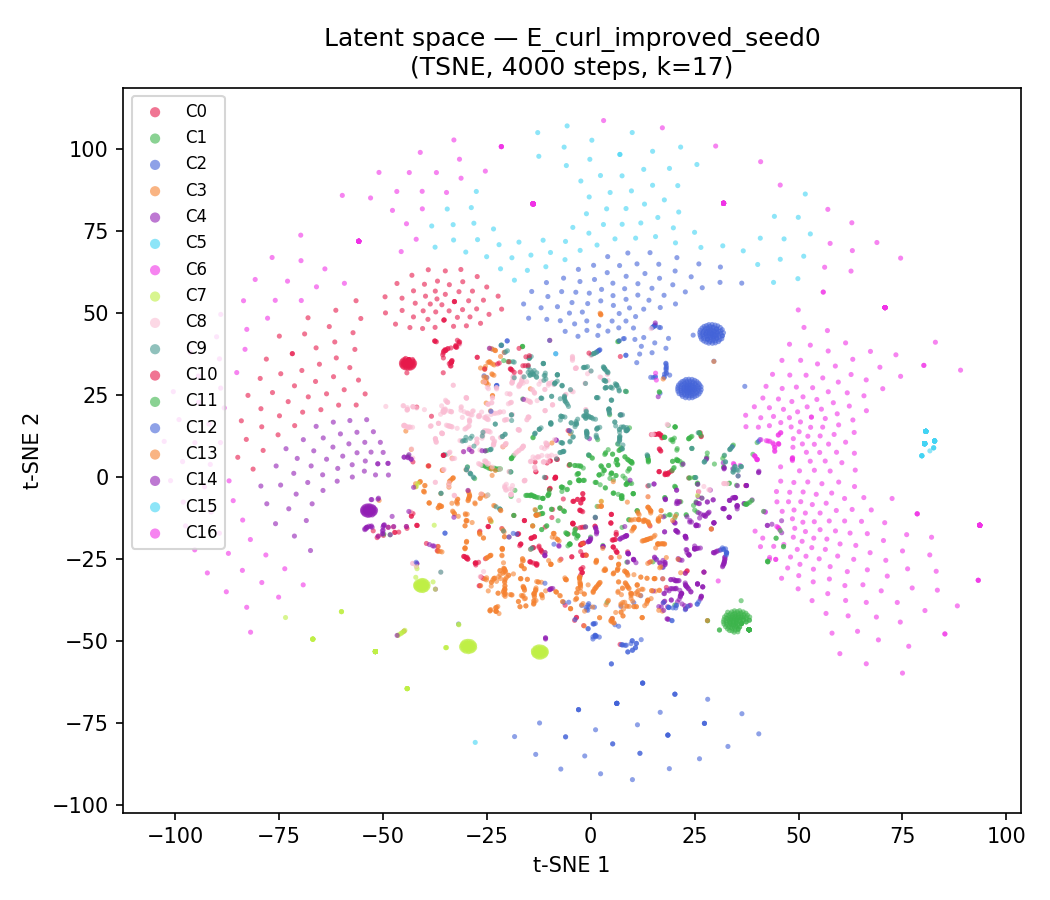
\includegraphics[width=0.72\textwidth]{figures/embedding_greedy_scatter.png}
    \caption{Two-dimensional t-SNE projection of latent embeddings from the
    trained \textsc{E\_curl\_improved} encoder under greedy rollout.
    Six $k$-means clusters are visible, corresponding to qualitatively distinct
    body configurations (see Figure~\ref{fig:boards}).}
    \label{fig:tsne}
\end{figure}

\begin{figure}[h]
    \centering
    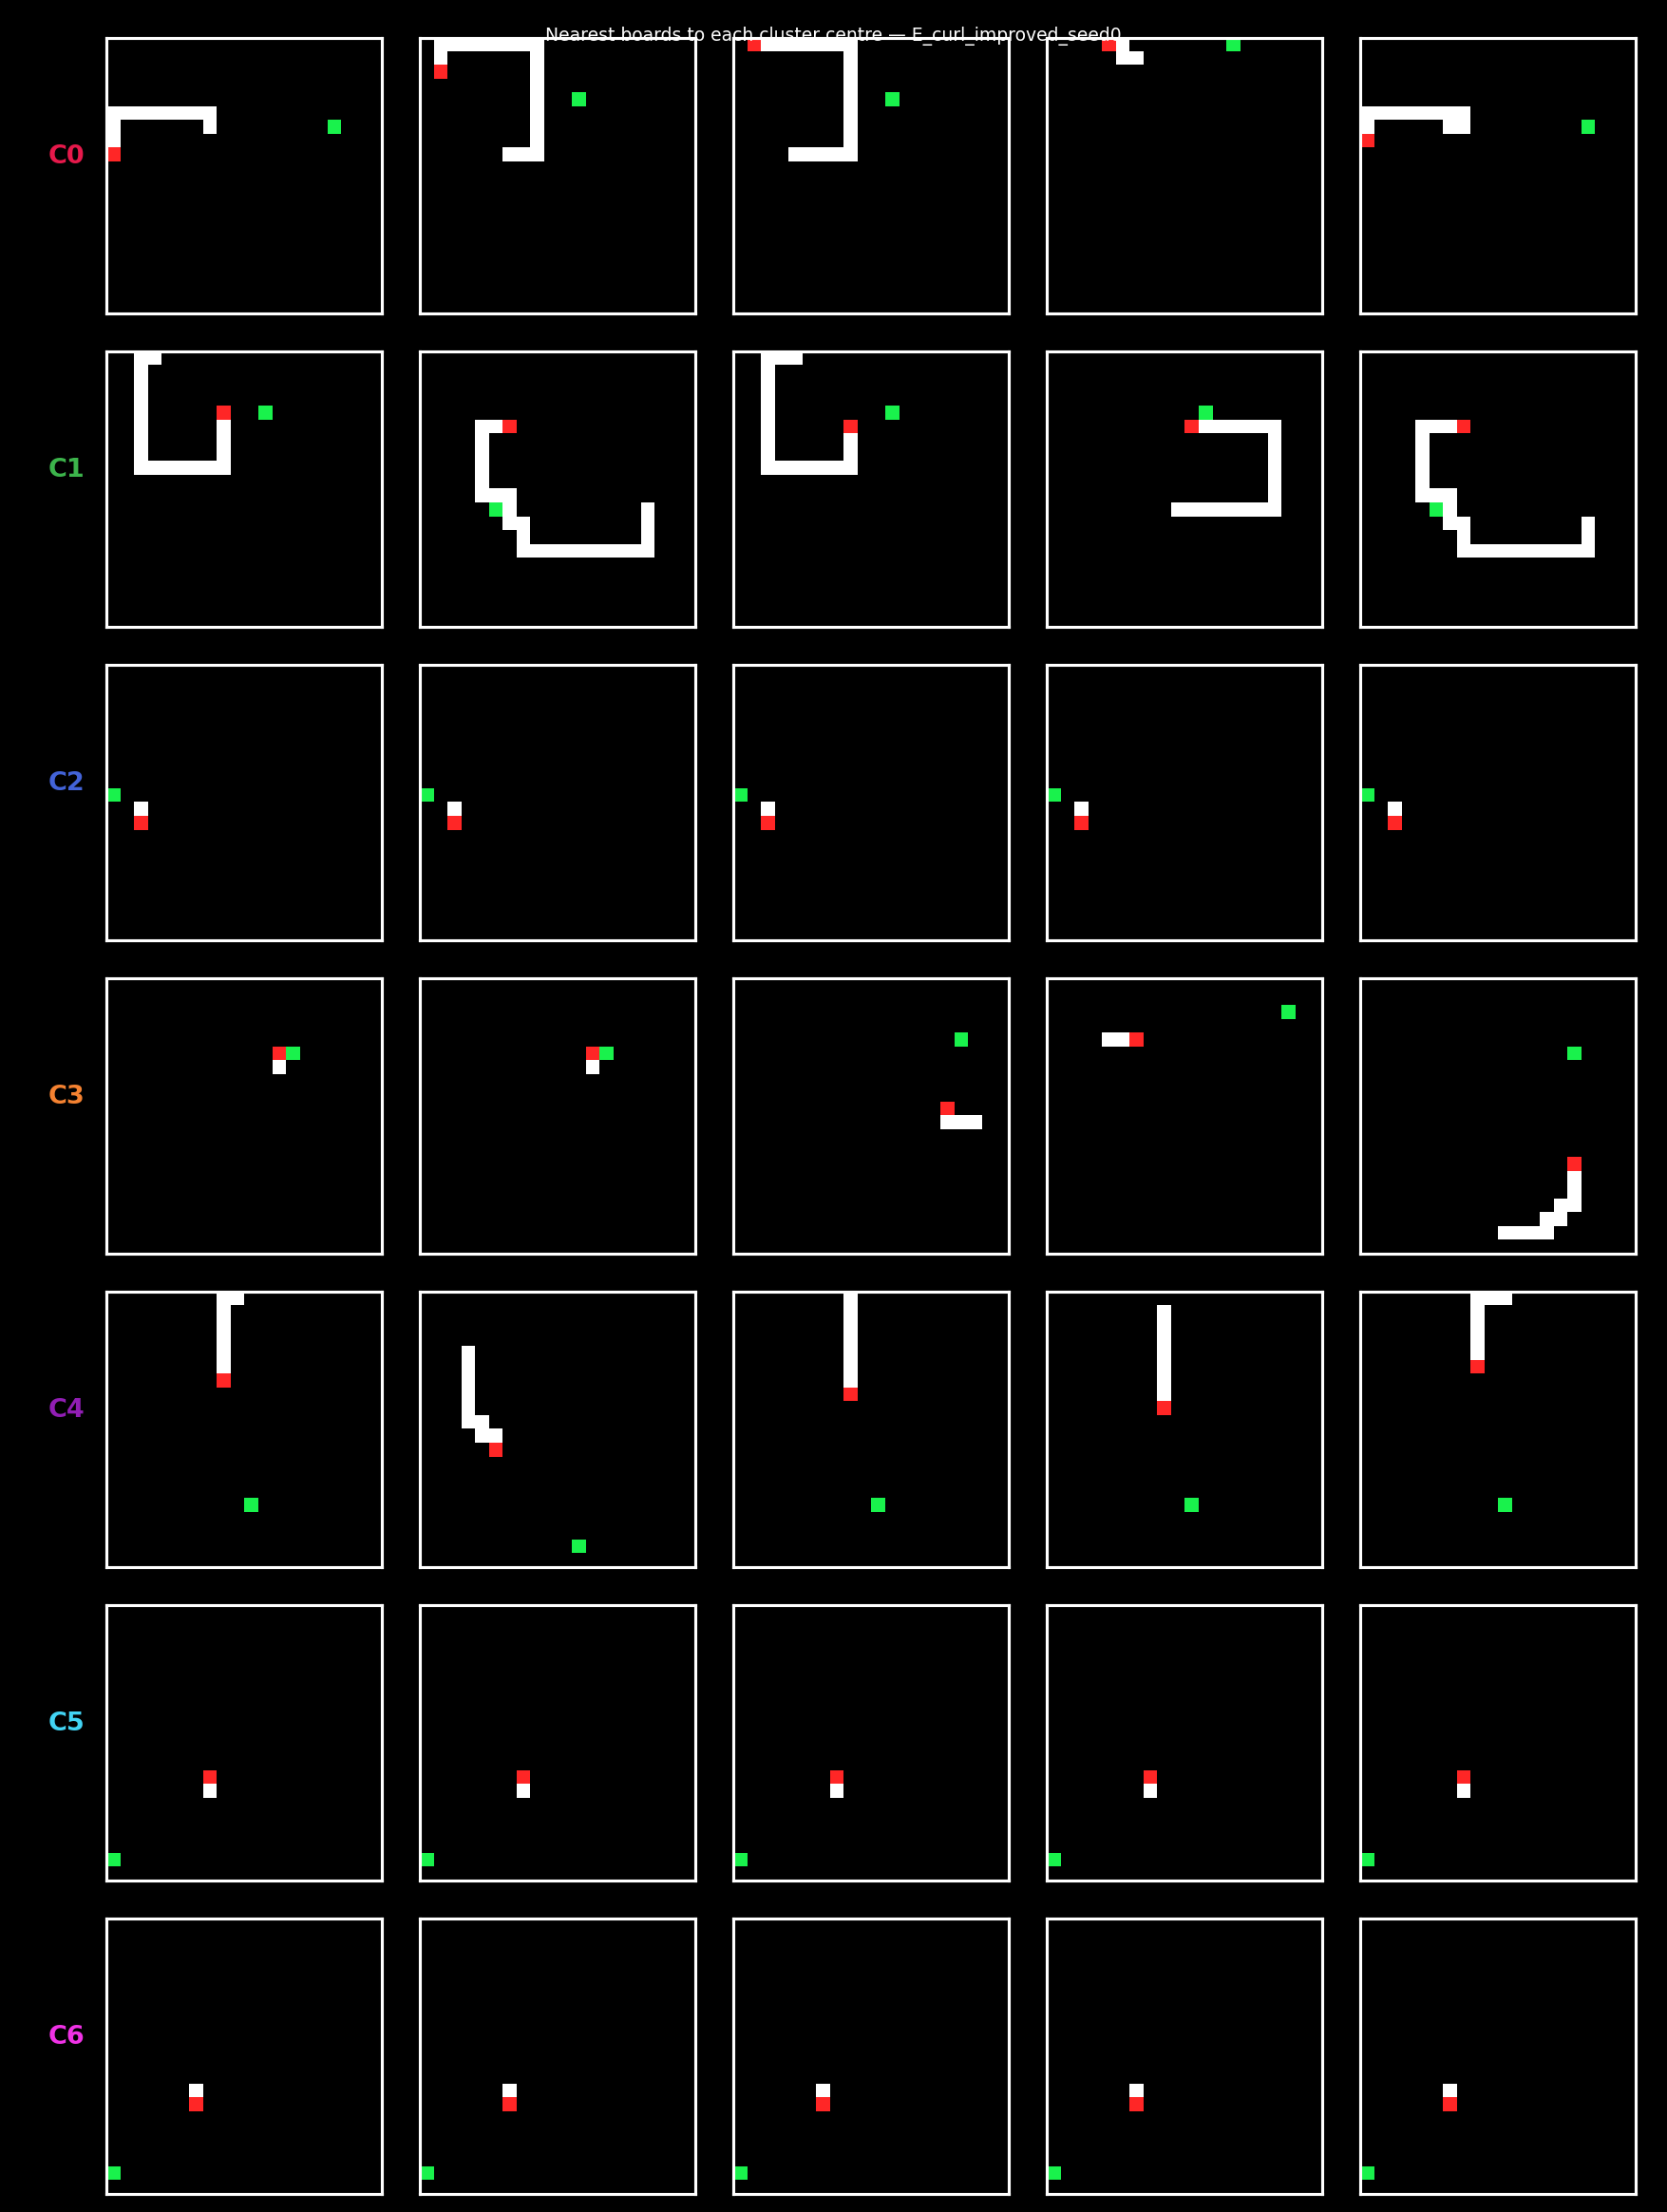
\includegraphics[width=\textwidth]{figures/embedding_greedy_boards_1.png}
    \caption{Nearest board states to cluster centres C0--C6.
    C0--C1 contain the longest, most complex bodies: U-shapes, hooks, and
    bracket-shaped configurations that require careful path planning to avoid
    self-collision.
    C2--C6 show progressively shorter bodies in various orientations,
    reflecting mid-game states.}
    \label{fig:boards1}
\end{figure}

\begin{figure}[h]
    \centering
    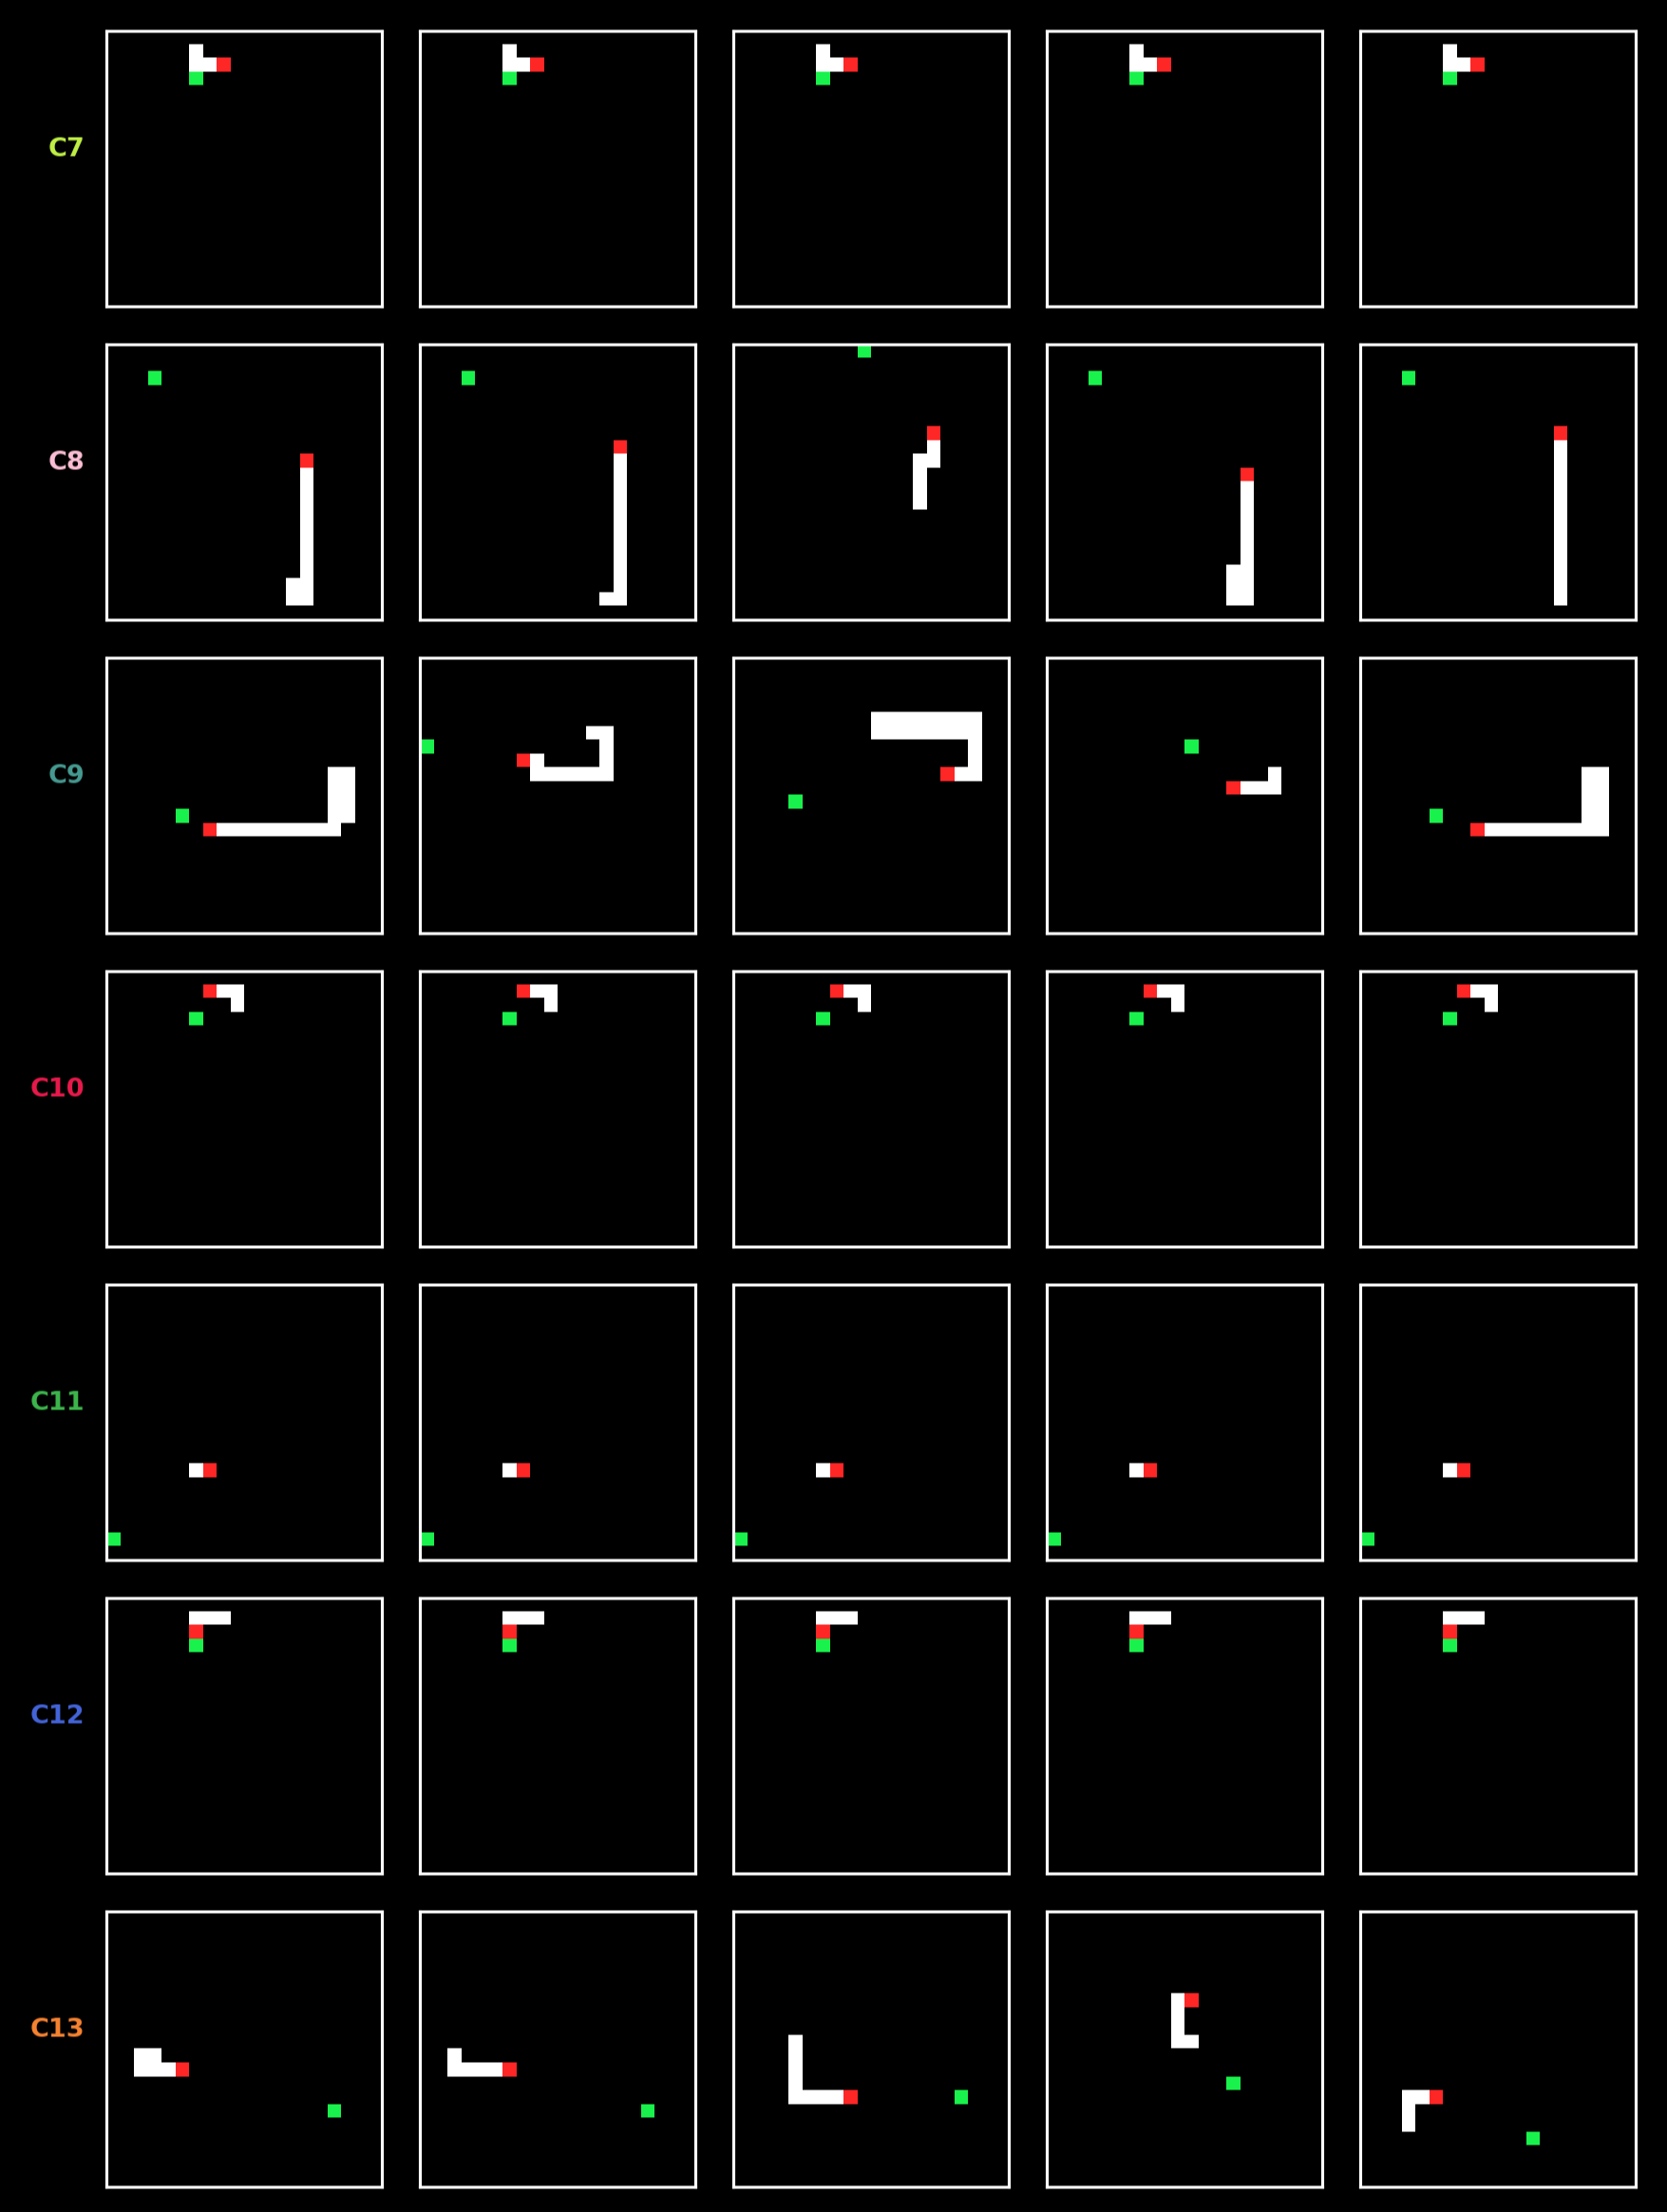
\includegraphics[width=\textwidth]{figures/embedding_greedy_boards_2.png}
    \caption{Nearest board states to cluster centres C7--C13.
    C8 groups long vertical bodies; C9 groups medium L-shaped bodies moving
    horizontally; C10 and C12 capture short angled configurations near the
    board edges.
    Within each cluster the body shape is consistent while the apple position
    varies — evidence that the encoder organises by structural body configuration
    rather than apple location.}
    \label{fig:boards2}
\end{figure}

\begin{figure}[h]
    \centering
    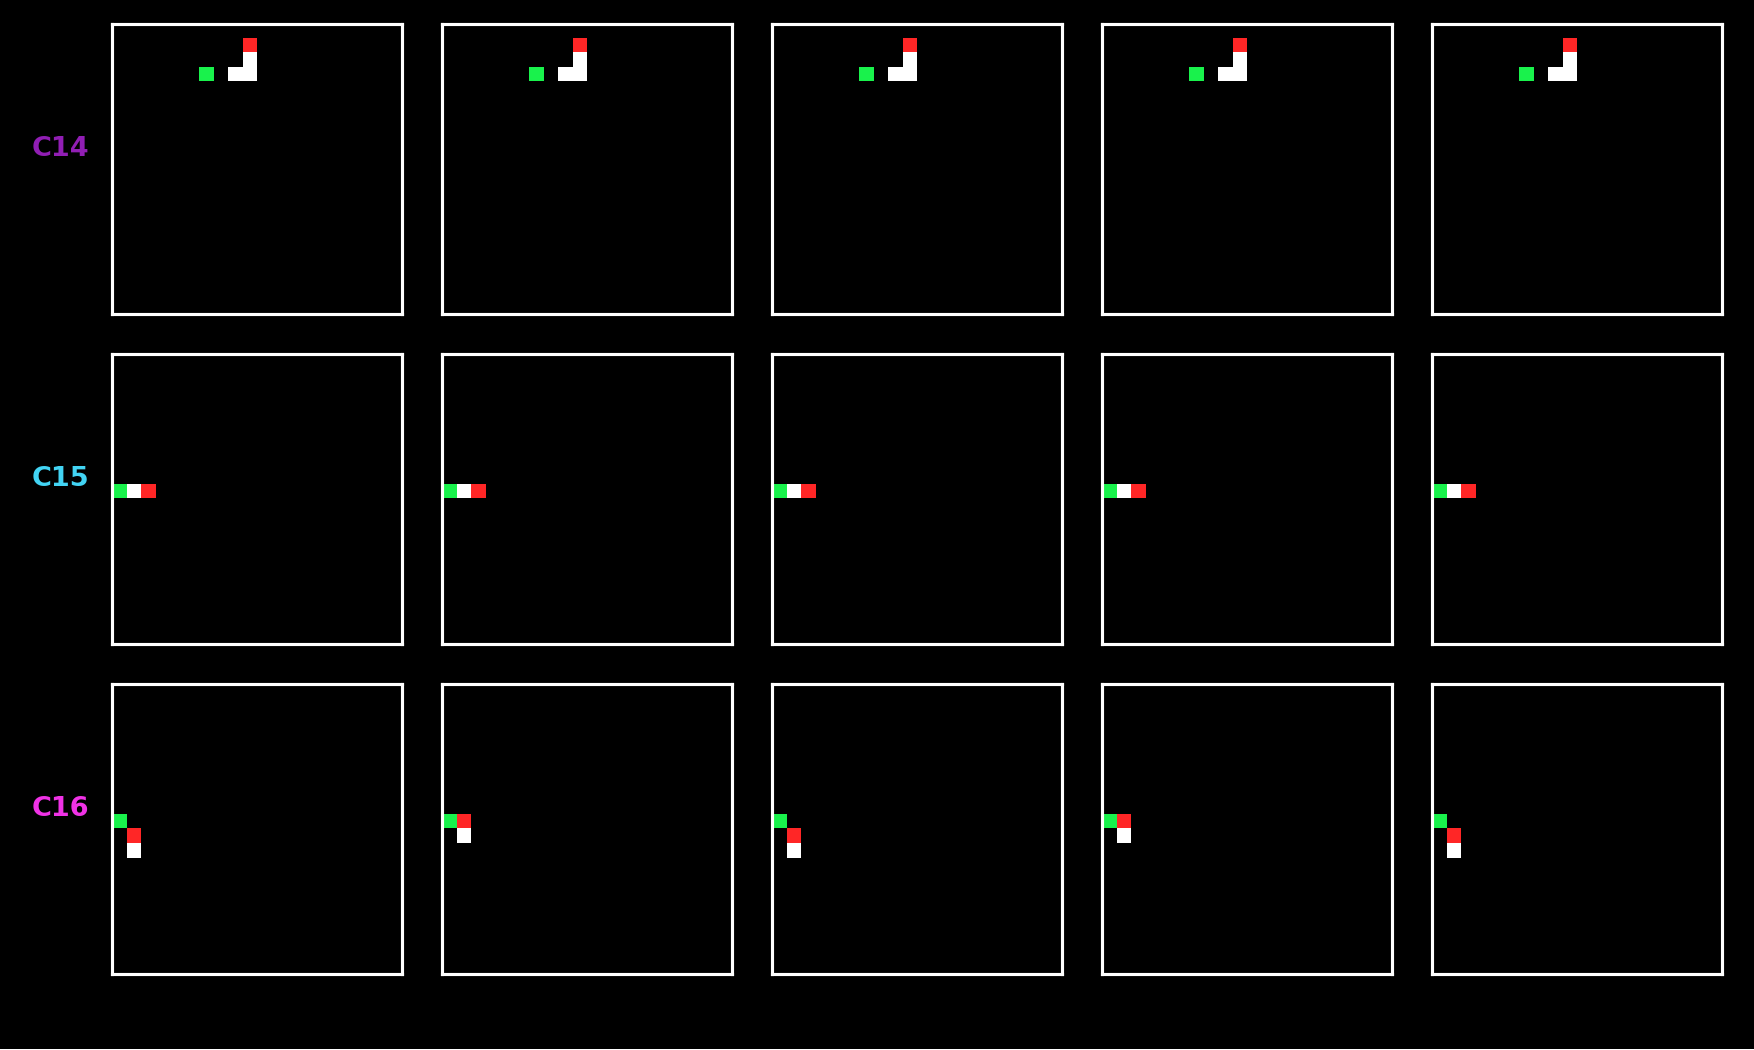
\includegraphics[width=\textwidth]{figures/embedding_greedy_boards_3.png}
    \caption{Nearest board states to cluster centres C14--C16.
    These clusters capture short early-game bodies (2--3 cells) with the apple
    in distinct relative positions: C14 groups states where the apple is
    above-left of the head, C15 groups states where the apple is directly
    to the left, and C16 groups states where the apple is below the head.
    Together, Figures~\ref{fig:boards1}--\ref{fig:boards3} show that the encoder
    separates states by body length at the coarse level, and by
    head-to-apple geometry at the fine level.}
    \label{fig:boards3}
\end{figure}

As shown in Figures~\ref{fig:tsne}~and~\ref{fig:boards1}--\ref{fig:boards3},
the encoder organises the latent space by body-shape structure at two levels
of granularity.
At the coarse level, long complex bodies (C0--C1: U-shapes, hooks, brackets)
separate clearly from medium bodies (C2--C13) and short early-game bodies
(C14--C16).
At the fine level, within each length stratum the encoder further distinguishes
states by head orientation and body direction.
Crucially, within each cluster the body shape is consistent while the apple
position varies freely across samples — confirming that the contrastive
objective has learned position-invariant structural features of the body,
precisely the representational property that motivated our choice of CURL
over the local-window baseline.

% ============================================================
\section{Discussion: Limitations and Failure Modes}
% ============================================================

\subsection{Gradient Instability at High Scores}

Despite the architectural improvements in \textsc{E\_curl\_improved}
(target network, Double DQN, $z_{\dim}=128$), training becomes noticeably
unstable once the snake's score approaches 30.
The symptom is intermittent spikes in the Q-loss, where the loss rises by
one to two orders of magnitude before recovering.

The root cause is the reward structure: a single apple-eating event returns
$+50$, which is an order of magnitude larger than the step-level shaping
rewards ($+3$ / $-1$).
When the snake reaches score 30, episodes become long enough that multiple
eating events can occur within a single trajectory, producing Q-targets with
much higher variance than early in training.
Gradient clipping (max-norm 10) prevents the worst parameter updates but
does not eliminate the instability; it limits the size of individual steps
rather than reducing the variance of the targets themselves.
A more principled remedy would be reward normalisation or the Huber loss in
place of MSE.

\subsection{Apple Signal Dilution at High Body Length}

A subtler failure mode emerges from the interaction between body length and
the contrastive objective.
The apple is represented as a single pixel on its own channel (1 out of 400
cells).
As the snake's body grows, the body pixels increasingly dominate the spatial
content of the image.
Consequently, the gradient signal that the InfoNCE loss provides for
discriminating states by \emph{apple location} diminishes relative to the
signal for discriminating by \emph{body shape}.

The practical effect is that at high body lengths the learned embedding $z$
encodes body configuration accurately but becomes less precise about apple
position.
The Q-function, receiving a less apple-informative $z$, issues less
responsive actions toward the apple — which contributes to the performance
plateau around score 30.
This is visible in the cluster boards (Figures~\ref{fig:boards1}--\ref{fig:boards3}):
long-body clusters (C3, C5) show consistent body shapes across samples,
whereas the apple position varies widely within the same cluster, indicating
that the encoder treats apple location as secondary information in these states.

The natural remedy is to concatenate the apple's $(x, y)$ coordinates
explicitly into the MLP stage of the encoder (alongside the existing
direction one-hot), ensuring that apple position is always precisely
represented regardless of body length.
We leave this modification to future work.

\subsection{Performance Gap Relative to the Local-Window Baseline}

The most striking result is the persistent gap between the contrastive
pixel-based agent and the hand-crafted local-window baseline.
Setup A reached a maximum score of 74 within 1{,}000 episodes, whereas
\textsc{E\_curl\_improved} achieved only 30 over 2{,}000 episodes.
We identify two structural factors as the principal contributors.

\textbf{Allocentric versus egocentric observation.}
The local-window encoder receives an observation already expressed in the
agent's egocentric frame: the $9\times9$ grid is always centered on the head,
so the same local configuration produces the same feature vector regardless
of absolute position.
The contrastive encoder operates on the full $3\times20\times20$ allocentric
grid, where the same local situation produces a different image depending on
where on the board it occurs.
Despite the random pad-and-crop augmentation being designed to encourage
position invariance, a pad of 2 (maximum spatial shift of 4 pixels) is
insufficient to fully bridge the gap between the allocentric and egocentric
settings.

\textbf{Representational complexity and apple signal dilution.}
As discussed above, the fixed $128$-dimensional latent vector must
simultaneously encode body shape and apple location.
At high body lengths, body shape dominates the pixel content of the
observation, causing apple-position information to be underrepresented in
$z$.
In the local-window setting this problem does not arise because the apple
direction is explicitly provided as a separate input feature.

Together, these factors suggest that closing the performance gap requires
not only more training episodes and a more stable training algorithm, but
also a fundamental change to the observation design — either an egocentric
global map, or an explicit positional encoding of the apple that makes its
location always precisely recoverable from $z$.

\begin{thebibliography}{9}
\bibitem{curl2020}
  A.~Srinivas, M.~Laskin, and P.~Abbeel,
  ``CURL: Contrastive Unsupervised Representations for Reinforcement Learning,''
  \emph{ICML}, 2020.
\bibitem{oord2018cpc}
  A.~van den Oord, Y.~Li, and O.~Vinyals,
  ``Representation Learning with Contrastive Predictive Coding,''
  \emph{arXiv:1807.03748}, 2018.
\bibitem{ddqn}
  H.~van Hasselt, A.~Guez, and D.~Silver,
  ``Deep Reinforcement Learning with Double Q-learning,''
  \emph{AAAI}, 2016.
\end{thebibliography}

\end{document}
